\chapter{Stand van zaken}
\label{ch:stand-van-zaken}

% Tip: Begin elk hoofdstuk met een paragraaf inleiding die beschrijft hoe
% dit hoofdstuk past binnen het geheel van de bachelorproef. Geef in het
% bijzonder aan wat de link is met het vorige en volgende hoofdstuk.

% Pas na deze inleidende paragraaf komt de eerste sectiehoofding.
%
%Dit hoofdstuk bevat je literatuurstudie. De inhoud gaat verder op de inleiding, maar zal het onderwerp van de bachelorproef *diepgaand* uitspitten. De bedoeling is dat de lezer na lezing van dit hoofdstuk helemaal op de hoogte is van de huidige stand van zaken (state-of-the-art) in het onderzoeksdomein. Iemand die niet vertrouwd is met het onderwerp, weet er nu voldoende om de rest van het verhaal te kunnen volgen, zonder dat die er nog andere informatie moet over opzoeken \autocite{Pollefliet2011}.
%
%Je verwijst bij elke bewering die je doet, vakterm die je introduceert, enz. naar je bronnen. In \LaTeX{} kan dat met het commando \texttt{$\backslash${textcite\{\}}} of \texttt{$\backslash${autocite\{\}}}. Als argument van het commando geef je de ``sleutel'' van een ``record'' in een bibliografische databank in het Bib\TeX{}-formaat (een tekstbestand). Als je expliciet naar de auteur verwijst in de zin, gebruik je \texttt{$\backslash${}textcite\{\}}.
%Soms wil je de auteur niet expliciet vernoemen, dan gebruik je \texttt{$\backslash${}autocite\{\}}. In de volgende paragraaf een voorbeeld van elk.
%
%\textcite{Knuth1998} schreef een van de standaardwerken over sorteer- en zoekalgoritmen. Experten zijn het erover eens dat cloud computing een interessante opportuniteit vormen, zowel voor gebruikers als voor dienstverleners op vlak van informatietechnologie~\autocite{Creeger2009}.

%	EFFECTIEVE LITERATUURSTUDIE

Dit hoofdstuk bestaat uit een uitgebreide literatuurstudie, waarin de kern van het probleem wordt opgesplitst in verschillende delen. In het eerste deel wordt er uitleg gegeven over JavaScript zelf en diens evolutie. Vervolgens volgt er een groot deel over de frameworks Node.js en Express, nadien bekijken we het belang van testen en monitoren van software en breiden we uit naar een analyse van dergelijke monitoringsoftware. In het tweede deel wordt er onderzoek gedaan naar de vraag van Kayzr: wat wordt er verwacht, welk inzicht moet er gegeven worden, welke features moeten worden uitgewerkt. 

\section{JavaScript}
\label{sec:javascript}

JavaScript is een programmeertaal gemaakt voor het web, waarmee statische websites kunnen omgezet worden naar dynamische en interactieve websites. Doordat het een enorm krachtige scripttaal is dat speciaal werd ontwikkeld om de functionaliteiten van een doorsnee webpagina gemaakt uit de talen HTML en CSS, uit te breiden, wordt het bijna onmogelijk om nog iets in te beelden dat niet geïmplementeerd kan worden m.b.v. JavaScript. De taal is weakly-typed, functioneel, event-driven en dynamisch (hierover volgt later meer uitleg). 

JavaScript bevat een bibliotheek van standaardobjecten samen met specifieke taalelementen zoals operatoren, controlestructuren, enz... Deze kern of 'core' kan makkelijk uitgebreid worden met extra objecten waardoor de taal eenvoudig kan aangepast worden aan verschillende omgevingen. Hierdoor wordt JavaScript regelmatig gespecificeerd als \textit{client-side JavaScript} en \textit{server-side JavaScript}. Client-side JavaScript wordt bijvoorbeeld gebruikt om de interactie met de gebruiker te verzorgen, zoals muiskliks, keyboard-hits en nog veel meer. Server-side JavaScript houdt zich eerder bezig met het achterliggende van een site, bijvoorbeeld om een webapplicatie te doen communiceren met een databank. Een zeer bekende en veel gebruikte server-side JavaScript dialect is Node.js, waarover later meer uitleg volgt. \autocite{Javascript2019}

\subsection{Tijdlijn van JavaScript}
\label{sec:jsTimeline}

JavaScript heeft een hele evolutie achter de rug. Ontstaan in mei 1995, wordt de taal na vele updates nog steeds dagelijks gebruikt en kan het wereldwijde web niet meer ingebeeld worden zonder. Brendan Eich, de auteur van de taal, werkte in 1995 samen met Netscape Communications, de makers van de eerste grote webbrowser (Netscape Navigator), om in hun browser een taal te implementeren waar webontwikkelaars gebruik van zouden kunnen maken. Java, een zeer zware programmeertaal met tal van functionaliteiten, was de eerste keuze van Netscape, maar Eich schreef uiteindelijk zijn eigen idee van een scripttaal uit in nog geen 10 dagen en overtuigde Netscape om die lichte, schaalbare en Java-complementerende taal te adopteren \autocite{Rangpariya2019}. Javascript, toen onder de naam Mocha en vervolgens LiveScript, was geboren en zette de wereld van webontwikkelaars op zijn kop.

Netscape bracht achteraf nieuwere versies van JavaScript uit, maar Microsoft dreigde die te onttronen. Niet zoveel later immers, bracht Microsoft Internet Explorer 3 uit met een eigen variant op JavaScript, namelijk JScript. Dit was een zware slag voor Netscape, aangezien Microsoft hen hierdoor zou inhalen. Tegelijk was het een grote stap in de evolutie van JavaScript zoals wij het nu kennen. Dat bracht echter problemen met zich mee, want bedrijven zouden telkens eigen versies van JavaScript uitbrengen wat voor veel compatibiliteitsproblemen zou zorgen. Uiteindelijk, in 1997, werd JavaScript 1.1 gestandaardiseerd dankzij het European Computer Manufacturers Association (ECMA) en werd JavaScript omgedoopt tot ECMAScript. \autocite{Wiley2016} Deze standaard, namelijk ES1 (versie 1), zou dan vertakkingen verhelpen. Implementaties van ECMAScript, waaronder JScript, ActionScript, maar dus ook JavaScript zelf, zouden dan telkens ECMAScript implementeren waardoor de kern van de varianten telkens hetzelfde blijft. Nu, in 2019, is JavaScript nog steeds enorm populair en implementeert die ondertussen al de 9e versie van ECMAScript: ES2018. Na ES5 is ECMASCRIPT overgeschakeld naar jaarlijkse releases, startend vanaf ES2015.

\subsection{Waarom JavaScript?}
\label{sec:jsWhy}

JavaScript is niet voor niets enorm populair, zelfs nog steeds na al die jaren, dankzij de vele voordelen dat de taal met zich meebrengt. En die lijst van voordelen wordt per iteratie alleen maar groter. Hieronder worden er enkele kernvoordelen opgesomd.

\subsubsection{Dynamisch en weakly-typed}
\label{sec:dynamic}

Een dynamisch getypeerde taal slaat op het feit dat het type van waarden kan veranderen tijdens uitvoertijd. Dat betekent bijvoorbeeld dat een variabele met als type string (een tekstvariable) plots kan gebruikt worden om een som te maken met een getal. Dit maakt uitvoertijd en compileertijd aanzienlijk sneller omdat er niet voortdurend controles moeten plaatsvinden. Dit zorgt voor hoge performantie, maar slechte nauwkeurigheid.

\begin{lstlisting}[style=ES6,
caption={Voorbeeld dynamisch getypeerde taal.},
label=code:dynamic]
foo = 10;	// Dit is een getal
bar = '10';	// Dit is een string
console.log(foo + bar); // Logt 20
\end{lstlisting}

\subsubsection{DOM-manipulatie}
\label{sec:DOM}
\begin{figure}[h]
	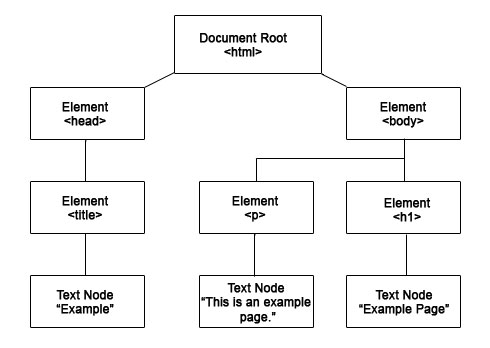
\includegraphics[width=\linewidth]{dom.jpg}
	\caption{Voorbeeld van een DOM structuur.}
	\label{fig:dom}
\end{figure}

De DOM, ofwel Document Object Model, is kortweg het skelet van een HTML-pagina. De structuur van het skelet beschrijft een boomstructuur, waardoor een element een ouder, broer, kind, kleinkind, achterkleinkind, enz... van een ander element kan zijn, zoals beschreven in \ref{fig:dom}. Het HTML-element is de wortel van de boom. Client-side JavaScript wordt grotendeels gebruikt om deze boomstructuur te manipuleren. Hierdoor kunnen we HTML-elementen toevoegen, verwijderen, stijlen wijzigen, enz... allemaal tijdens uitvoertijd. \textcite{Kantor2017}

\subsubsection{Prototype-based}
\label{sec:prototypeBased}

In JavaScript kan een object eigenlijk aanzien worden als een array\footnote{Een array is een variabele dat meerdere objecten kan opslaan.}. Hierdoor zijn de eigenschappen van een object zeer toegankelijk en kunnen deze ook makkelijk tijdens uitvoertijd aangepast worden. Ook kunnen er op deze manier makkelijk eigenschappen aan bestaande objecten worden toegevoegd. In JavaScript wordt gebruik gemaakt van de 'dot-notatie' of van de 'haakjesnotatie'. 

\begin{lstlisting}[style=ES6,
	caption={Voorbeeld van de dot-en haakjesnotatie.},
	label=code:dot]
	foo.bar = 10;
	foo['bar'] = 10;
	const bar = foo.bar;
	foo['bar2'] = bar;
\end{lstlisting}

\subsubsection{Event-driven}
\label{sec:eventDriven}

JavaScript is event-driven, wat betekent dat de code vooral kijkt naar acties van de gebruiker. Bijvoorbeeld: Wanneer een gebruiker op een knop klikt, wil je dat met een animatie de knop heen en weer beweegt of tekst op je scherm verschijnt of een request naar een server wordt gestuurd. 

\begin{lstlisting}[style=ES6,
caption={Functionele programmeerstijl.},
label=code:func]
//Pre-functioneel
const verdubbelen = nummers => {
const verdubbeld = [];
for (let i = 0; i < nummers.length; i++) {
	verdubbeld.push(nummers[i] * 2);
}
return verdubbeld;
};

//Functioneel
const verdubbelen = nummers => nummers.map(n => n * 2);
\end{lstlisting}

\subsubsection{Functioneel}
\label{sec:functional}

Sinds ES2015 is JavaScript niet enkel en alleen een object-georiënteerde taal, maar ook een functionele taal. JavaScript was zeer snel met het introduceren van de nieuwe functionele programmeerstijl (waaronder de populaire arrow-functions). Dit vergemakkelijkte de taal aanzienlijker, aangezien veel minder code geschreven moest worden om hetzelfde resultaat te bereiken.

\subsubsection{Universeel}
\label{sec:universal}

JavaScript wordt sinds ES5 ondersteund door alle moderne browsers! Of er nu in Chrome, Firefox, Safari, Edge of het oude Internet Explorer\footnote{Internet Explorer wordt niet meer verder ontwikkeld, dus ondersteunt het enkel ES2015.} wordt gesurft, ze ondersteunen allemaal JavaScript. Door de console in de browser te openen, kan er zelfs al geprogrammeerd worden.




\section{Node.js}
\label{sec:nodeJs}

Node.js is een open-source JavaScript runtime-omgeving die wordt gebruikt voor server-side toepassingen. Node.js maakt het mogelijk (of eerder \textit{makkelijker}) om JavaScript nu ook te gebruiken buiten het maken van websites. Aangezien JavaScript zo'n krachtige taal is, hadden de ontwikkelaars van Node.js één ding in gedachten: JavaScript niet enkel voor browsers, maar ook voor alleenstaande applicaties. Sindsdien evenaart JavaScript andere scripttalen voor backend\footnote{Backend is een ander woord voor software die niet aan de eindgebruiker wordt getoond. Het tegenovergestelde van backend is frontend. Letterlijk het programmeren van de voor-of achterkant van software. } toepassingen, zoals Python. \textcite{Patel2018}

\subsection{Tijdlijn van Node.js}
\label{sec:nodeTimeline}
Node.js' verhaal start in 2009, toen de ontwikkelaar Ryan Dahl een probleem ondervond met Apache Http Servers. 

Zoals beschreven in \autocite{Chaniotis2015}, was (en is in grote mate nog steeds) Apache HTTP, in combinatie met PHP, jarenlang de go-to-taal om webapplicaties te laten communiceren met databases en server-side functionaliteiten toe te voegen aan \linebreak webapplicaties, zoals authenticatie, file-en-ftpservers, logging en nog veel meer. PHP is echter nooit ontwikkeld geweest om hedendaagse, complexe webapplicaties te schrijven. Ten tweede was Apache niet in staat om te schalen naar meerdere processorkernen, waardoor de performantie enorm daalde. PHP in combinatie met Apache was gewoonweg niet geschikt voor de volgende generatie webapplicaties. Andere struikelblokken zijn cross-platform mobiele applicaties en real-time communicatie.

Applicaties worden in toenemende mate ontwikkeld met cross-platform compatibiliteit in het achterhoofd, aangezien de toestroom van verschillende nieuwe besturingssystemen en apparaten het meer en meer ingewikkeld maakt om native apps\footnote{Native Apps zijn applicaties die gemaakt worden voor één besturingssysteem. Bv: Android, IOS, Windows.} te ontwikkelen. Hierdoor worden bibliotheken en frameworks ontwikkeld zoals React Native, Flutter, Xamarin, Ionic, PhoneGap, enz... die deze nadelen kunnen overbruggen. Deze zijn echter zo krachtig geworden en schenken zoveel nieuwe voordelen, dat server-side talen en frameworks zoals Apache HTTP/PHP eerder een knelpunt vormden. 

Real-time communicatie is nog een factor die niet ondersteund wordt door Apache. Apache was niet ontwikkeld om berichten te sturen naar de client-side. In de wereld van vandaag, waarin sociale media nog nooit zo'n grote invloed hebben gehad op ons dagelijks leven, is het haast ondenkbaar dat real-time communicatie niet zou kunnen bestaan. 

Al deze voorgaande elementen hebben bijgedragen tot de ontwikkeling van Node.js. Het project van Dahl werd met open armen ontvangen. Na enkele struikelblokken zag Node.js in 2011 voor het eerst het licht en wordt het nu gebruikt in vele moderne applicaties. Ook vandaag is het steeds één van de meest gegeerde vaardigheden van een programmeur. \autocite{Patel2018}

Hoewel Apache en PHP nog steeds overduidelijk op plaats één staan, hebben ze hun succes enkel nog te danken aan bedrijven die op verouderde software werken, en aan hun populariteit bij senior ontwikkelaars. PHP blijft een geliefde taal bij velen, maar in \ref{fig:trend} zien we dat Node.js's populariteit duidelijk die van Apache aan het inhalen is. \autocite{SimilarTech}

\begin{figure}[h]
	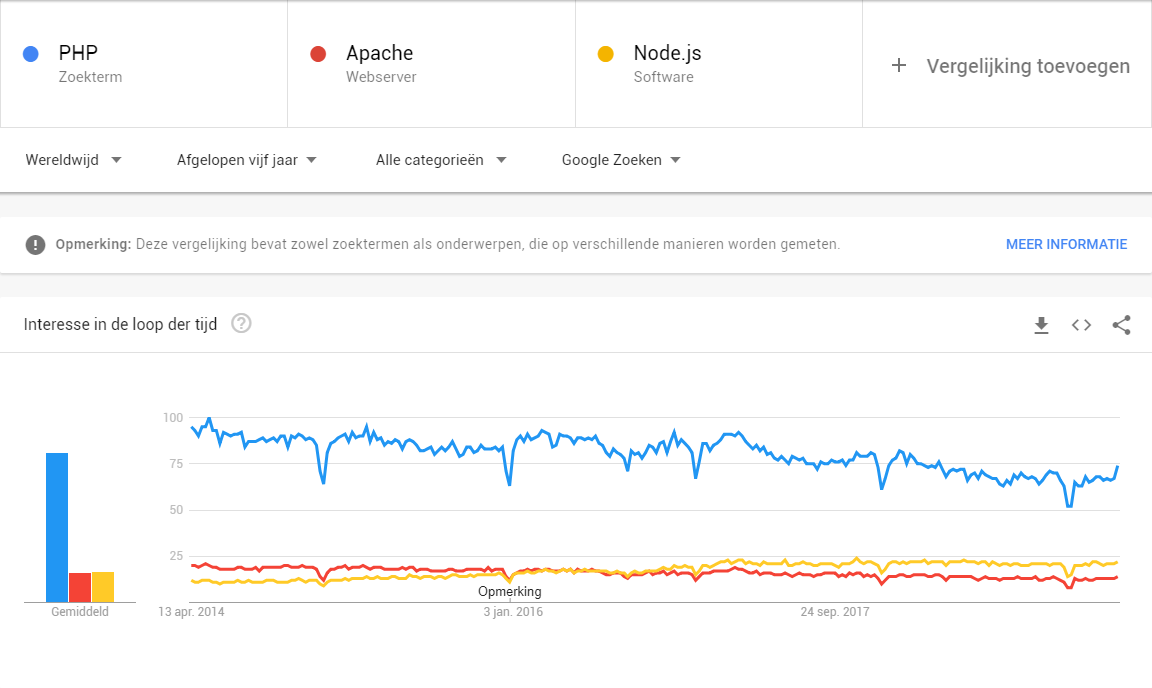
\includegraphics[width=\linewidth]{trend.png}
	\caption{Google searches van PHP (blauw), Apache (rood) en Node.js (geel) in de afgelopen 5 jaar.}
	\label{fig:trend}
\end{figure}

\subsection{Waarom Node.js?}
\label{sec:whyNode}
Node.js is reeds een volwassen server-side framework. Youtube, Yahoo, Google, Amazon, Netflix, eBay, Reddit, LinkedIn, Paypal, Github, Forbes, Walmart, Uber, NASA, Slack,.. zijn slechts enkele van de duizenden websites die overgeschakeld zijn naar Node.js. En dit zijn geen kleine namen.

Illustrator \textcite{Mehmet2016} toont duidelijk de voordelen van Node.js aan. LinkedIn kon zijn 15 servers reduceren naar slechts 4 en ondertussen de verkeerscapaciteit nog eens verdubbelen. Walmart kon al zijn client-side JavaScript processing naar zijn servers verplaatsen wat voor een enorme performantieboost zorgde, en eBay kon zijn verkeerscapaciteit enorm verhogen en het verbruik substantieel verlagen. De voordelen en functionaliteiten worden hieronder nog eens opgesomd zoals aangegeven door \textcite{Chandrayan2017}.

\subsubsection{Nieuw}
\label{sec:new}

JavaScript is relatief gezien een nieuwe taal die voortdurend geüpdatet wordt, in tegenstelling tot de traditionele server-talen zoals Python, PHP, enzovoort. Vele dialecten van JavaScript (zoals TypeScript, CoffeeScript, ClojureScript,...) compileren gewoonweg in JavaScript, waardoor overschakelen heel eenvoudig wordt. Doordat Node.js ook in JavaScript geschreven is, maakt dit het zowel voor de frontend-ontwikkelaar als voor de backend-ontwikkelaar makkelijker om client-en server-side dichter bij elkaar te brengen. \autocite{ExpressMozilla}

\subsubsection{Asynchroon}
\label{sec:async}

Node.js is sterk afhankelijk van asynchrone en continue programmeerstijl. I/O-bewerkingen worden uitgevoerd door middel van oproepen naar asynchrone functies waarbij een callback moet worden doorgegeven om aan te geven hoe de berekening wordt voortgezet zodra de genoemde I/O-bewerking asynchroon is voltooid. Het Node.js executiemodel bestaat uit een hoofdgebeurtenislus die wordt uitgevoerd op een single-threaded proces. Met behulp van deze \textit{event loop} moet een Node.js server nooit wachten op antwoord. Het kan gewoon blijven doordraaien na een oproep van een API Call en - dankzij een notificatiesysteem - op een later moment het antwoord terugsturen. Dit maakt Node.js enorm schaalbaar, in tegenstelling tot Apache dat slechts een gelimiteerd aantal threads kan starten om handelingen uit te voeren.

Het is daarom niet altijd makkelijk om dat soort frameworks te debuggen, en het wordt uiteindelijk een uitdagende taak. Gelukkig zijn hiervoor dan ook weer verschillende hulpmiddelen en tools uitgebracht om dit te vereenvoudigen. Zoals vermeld in ~\autocite{Runtime2017}, kan asynchrone code subtiele bugs opleveren die niet meteen zichtbaar zijn. Hier is nog niet echt onderzoek naar gedaan. Waar er honderden vergelijkende studies bestaan over de frameworks zelf en of Node.js een goede optie is, zijn er geen of amper studies over de beste manier om dit te debuggen en hoe men dit het best aanpakt. ~\autocite{Runtime2017} vertelt ons meer over het identificeren van schaalbaarheidsproblemen en het aanreiken van mogelijke oplossingen. Ze maken gebruik van parametrische uitdrukkingen voor runtime monitoring van Node.js toepassingen, maar ze geven toe dat dit nog maar de eerste stap is en dat hier nog meer onderzoek naar kan gedaan worden. Hierop wordt later in dit onderzoek dieper ingegaan.

\subsubsection{Performant}
\label{sec:fast}

Google Chrome's JavaScript engine, V8, is bijzonder snel. Dahl heeft dit verder ontwikkeld voor Node.js, wat het framework enorm performant en efficiënt maakt in het compileren en uitvoeren van code. Veel sneller dan Python, Ruby of Perl.

\subsubsection{npm}
\label{sec:npm}

Node.js kent een enorm bloeiende community. Node Package Manager, ofwel npm, is een onderdeel van Node.js en komt meegeleverd bij de installatie. Via npm kan men uit honderdduizenden pakketjes kiezen om een JavaScript/Node project in één oogwenk makkelijk uit te breiden met extra functionaliteiten. Dagelijks worden er nieuwe pakketjes toegevoegd aan de package manager. Dat is slechts één van de redenen waarom Node.js zo populair is, aangezien het ontwikkelen van een webapplicatie enorm wordt vereenvoudigd.   

\section{Express}
\label{sec:express}

\subsection{Waarom Express?}
\label{sec:whyExpress}

\textcite{ExpressMozilla} maakt ons echter duidelijk dat niet alles rechtstreeks door Node.js wordt ondersteund. Als men bijvoorbeeld aan een webapplicatie routing wenst toe te voegen, zoals HTTP \textsl{GET, POST, PUT, DELETE,} enzovoort... of URL-paden met specifieke requests, statische bestanden weergeven... moet men die code zelf schrijven. Herinner echter het npm-systeem van Node.js. Eén van die honderdduizenden pakketjes is Express. Het is veruit \textit{het} populairste Node framework en is zelfs de grondlegger van duizenden andere pakketjes. Express wordt daarom door bedrijven, waaronder Kayzr, dan ook vaak in combinatie gebruikt met Node.js.

\subsubsection{Request Handlers}
\label{sec:reqHandlers}

Dankzij Express wordt het zeer gemakkelijk om routering in een applicatie toe te voegen. Indien een GET request gemaakt wordt in de frontend naar een bepaalde URL, is dit zeer gemakkelijk om op te vangen m.b.v. Express. Voor elk soort request en elk type URL kan Express logica uitvoeren en code makkelijk verder delegeren.

\subsubsection{Views}
\label{sec:expressViews}

Express kan statische bestanden zoals HTML, CSS en afbeeldingen laten weergeven in de browser dankzij render engines. Makkelijk om bijvoorbeeld foutpagina's te weergeven.

\subsubsection{Modulair}
\label{sec:expressModularity}

Modulariteit is een kerneigenschap van Express. Express is \textit{unopinionated}, wat wil zeggen dat er niet echt een gouden regel is om een doel in Express te bereiken. Doelen kunnen op meerdere manieren bereikt worden, waardoor het makkelijker is voor ontwikkelaars om een bepaalde taak uit te voeren. Dankzij modulariteit kan het framework ook volledig naar wens ingesteld worden; van poorten en routers, het instellen van een databank tot het toevoegen van Express middleware. 

\subsubsection{Middleware}
\label{sec:expressMiddleware}

Wellicht de krachtigste eigenschap van Express is het gebruik kunnen maken van middleware. Middleware wordt voortdurend gebruikt in Express. Wanneer een request binnenkomt, wordt deze doorgestuurd door nul, één of meerdere middleware die elk iets doen met de request, tot deze uiteindelijk wordt afgehandeld. De volgorde waarin een request de middleware doorloopt, is volledig afhankelijk van de programmeur. Net zoals Node.js, kent Express ook een enorm grote bibliotheek aan middleware die men kan gebruiken in een applicatie en eveneens helemaal verkrijgbaar is via npm. Hierdoor kunnen ontwikkelaars zelf hun middleware schrijven, bestaande middleware downloaden en deze inpluggen in hun applicatie. Middleware kan gaan van Http-request loggers tot cookie-parsers en veel meer. De mogelijkheden zijn praktisch oneindig. Foutmeldingen zijn een goed voorbeeld van Express Middleware. Wanneer ergens iets fout gaat, roept Express de Error-Handler op, die dan zelf de request afwerkt. Monitoringtoepassingen in Node.js maken vaak gebruik van middleware. Hierover volgt meer info in het volgende hoofdstuk.

\begin{minipage}{\linewidth}
	\begin{lstlisting}[style=ES6,
						caption={Express code flow voorbeeld.},
						label=code:expressexample]
	const express = require('express');
	const app = express();
	
	// An example middleware function
	const a_middleware_function = function(req, res, next) {
	// ... perform some operations
	// Call next() so Express will call the next middleware function in the chain.
	next();
	}
	
	// Function added with use() for all routes and verbs
	app.use(a_middleware_function);
	
	// Function added with use() for a specific route
	app.use('/someroute', a_middleware_function);
	
	// A middleware function added for a specific HTTP verb and route
	app.get('/', a_middleware_function);
	
	app.listen(3000);
	\end{lstlisting}
\end{minipage}	
	
Middleware schrijven is op zich niet moeilijk. Men kan een enkele functie schrijven, of een heel takenpakket, die men dan als het ware injecteert in een request afhandeling. In een middleware functie verkrijgt men dan een req object, dat van de router kan komen of van een andere middleware, waar dan iets mee kan gedaan worden. Wanneer alles is uitgevoerd, roept de middleware de next-functie op, die dan het nieuwe res, of result, object doorstuurt naar de volgende middleware. Het kan ook zijn dat de middleware de next-functie niet oproept, wat betekent dat dit de laatste stop was van de router. Deze methodologie is gevisualiseerd in figuur \ref{fig:middleware}.

\begin{figure}[h]
	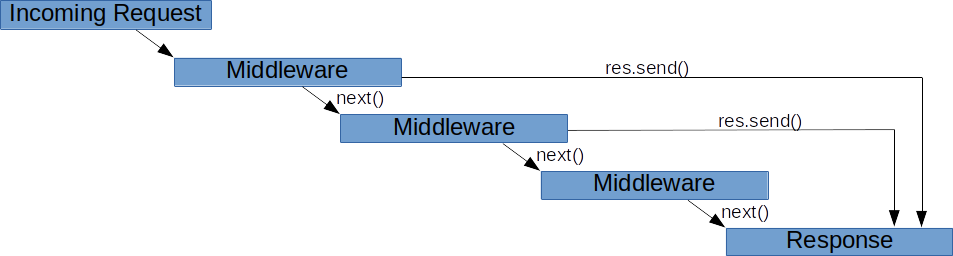
\includegraphics[width=\linewidth]{middleware.png}
	\caption{Schema van de werking van middleware, gebruikt van \cite{middleware}}
	\label{fig:middleware}
\end{figure}

\pagebreak
\section{Testen en Monitoring}
\label{sec:testAndMonitoring}

Testen schrijven. Of men nu alleen aan software werkt, of in team in een bedrijf, elke programmeur met gezond verstand zal kunnen vertellen over het belang van testen schrijven. Iets waar vaak wordt tegenop gezien, maar nodig is om een geslaagd, werkend product op te leveren. Meer en meer bedrijven gaan dit dan ook verplichten in hun implementatieproces. 

Testen en monitoring zijn twee termen die dicht bij elkaar horen. Door testen te implementeren kan men kwaliteitsvollere code schrijven, fouten sneller opsporen en is de software een pak robuuster. Het toevoegen van nieuwe functionaliteiten kan de code niet meer breken en daardoor kan de software langer meegaan. 

\subsection{Agile Testing}
\label{sec:agile}

Agile testing is een methodologie, ontstaan rond 1990, waarin software incrementeel en iteratief wordt uitgewerkt en die op de dag van vandaag in vele bedrijven wordt gehanteerd. Vooraleer er effectieve code wordt geschreven, zullen er eerst testen uitgewerkt worden, waarop men dan de code gaat schrijven. Zo verkrijgt men code die robuust, aanpasbaar en efficiënt is. Tijdens elke iteratie van het projectproces zullen er nieuwe testen worden geschreven en oude testen worden aangepast. Zo moet men telkens maar kleine gedeeltes code aanpassen of schrijven. Een goede handhaving van agile testing doet niet alleen de slaagkansen van het project vergroten, het kan het project ook goedkoper maken en de effectieve loopduur stabiel en klein houden.
Per sprint, of ontwikkelcyclus, worden er telkens eerst testen geschreven voordat men dan uiteindelijk begint met programmeren. \autocite{CHAKRAVORTY2014536}

Dit kan echter ook problemen met zich meebrengen. Agile vergt voorbereiding. \textcite{CHAKRAVORTY2014536} vertelt ons dat de kost en tijd van het project uit balans kunnen geraken telkens wanneer de klant iets wil veranderen. Daardoor komt er veel werk op de programmeurs te liggen. In \autocite{Borland2012} wordt dit ook nog eens samengevat. Veel bedrijven passen de agile methodologie toe, maar niet de agile testing. Dit komt omdat in agile de verantwoordelijkheid om beslissingen te nemen naar het team van ontwikkelaars wordt verschoven. Dat breekt met de traditionele watervalmethode waar de belangrijkste keuzes door management en niet door het team worden genomen. Dit breekt ook met de traditionele hiërarchische structuur waarin bedrijven werken. Het management verliest een deel van de controle over de richting van hun projecten. Het is dus veilig om te zeggen dat het implementeren van de agile methodiek niet alleen het werkproces van het bedrijf wijzigt maar ook de mentaliteit van het bedrijf. Veranderingen in een bedrijf gaan traag vooruit, zeker wanneer het een complete mentaliteitsverandering vergt. Daarom dat er veel bedrijven zijn die ervoor opteren om de agile methodiek slechts gedeeltelijk te implementeren. Zo laten ze een paar minder belangrijke componenten van de agile methodiek achterwege zoals bijvoorbeeld agile testing. Dit kan verklaren waarom er niet zo veel bedrijven zijn die agile testing effectief implementeren. Een andere grote hindernis bij agile testing is dat er niet veel tools bestaan die geavanceerde testingmethodes ondersteunen.

Wat men ook in de afgelopen tien jaar meer en meer terugziet, is de problematiek van het continu releasen van software. Software-reuzen zoals Google, Facebook, Mozilla, enzovoort... kozen ervoor om software telkens opnieuw uit te brengen in zeer korte periodes, ook wel \textit{rapid releases} genoemd. Mozilla kende bijvoorbeeld oorspronkelijk een release-cyclus van maanden, waarin elke grote versie vele nieuwe dingen met zich meebracht. Vanaf Firefox 5.0 zijn ze overgeschakeld naar een rapid release systeem. Daardoor brengen ze nieuwe, maar kleinere updates om de 6 weken uit. Dit kent zijn voordelen, maar echter ook zijn nadelen in het test-proces. Aangezien er aan een steeds hoger tempo moet uitgebracht worden, moeten testen meer geautomatiseerd worden, wordt er minder getest en is de software minder robuust. Hierdoor treden er sneller fouten op ~\autocite{Maentylae2013}. Kayzr kampt met dezelfde problemen. Daarom is er steeds meer nood aan monitoringtoepassingen die de duur van het debugproces van zo'n rapid release model aanzienlijk kunnen doen verminderen. Hierover volgt later meer info. 

\subsection{Soorten Agile Testing}
\label{sec:kindsOfTesting}

Er bestaan natuurlijk verschillende manieren om te testen, maar het wordt grotendeels opgesplitst in drie categorieën: unit testing, integratietesting en systeemtesting. Er zijn er nog andere: sanity testing, smoke testing, interface testing, regression testing, end to end testing, performantietesting,... zijn allerlei soorten opgesomd door \textcite{Pittet}. Dit zijn slechts de functionele testen. Men heeft ook niet-functionele testen, die dan in verband staan met andere aspecten van het project, zoals beveiliging en lokalisatie (taal),... Dan wordt er nog eens gekozen of men deze soorten testen wenst te automatiseren of niet. Daarin kruipt meer tijd, maar goed geschreven geautomatiseerde testen zijn een sleutelcomponent tot continue integratie en releases. Hier wordt echter niet verder in detail op ingegaan aangezien dit niet tot de scope van het onderzoek behoort.

\section{Monitoring}
\label{sec:monitoring}

Monitoring is een proces om de info en metriek te analyseren van een lopend proces. Zo kan monitoringsoftware er op letten dat alles verloopt volgens de afspraken, en indien dit niet het geval is, actie ondernemen ~\autocite{Rouse2018}. 

\subsection{Hoe werkt monitoring?}
\label{sec:howMonitoringWorks}

Real-time monitoring is een monitoringtechniek die dagelijks gebruikt wordt in de IT-wereld. Zo'n proces kan data verzamelen door voortdurend checks te doen op de lopende software, zoals het opvragen van CPU-verbruik, geheugenverbruik, foutmeldingen controleren,... Monitoringsoftware kan gebruik maken van \textit{agenten}, die dan specifiek geprogrammeerd kunnen worden om op een intelligente manier zaken te onderzoeken en desnoods af te handelen (bijvoorbeeld: een specifieke fout die opduikt).

Dankzij monitoring kan een applicatie draaiende gehouden worden, of kan een IT-medewerker tijdig opgeroepen worden om fouten op te sporen. Monitoring kent ook andere voordelen, zoals het verzamelen van data die dan gebruikt kan worden voor andere doeleinden, bijvoorbeeld voor de marketing-of managementafdeling. 

\texttt{vb: Stuur telkens een bericht naar de Administrator wanneer een IP-adres uit Amerika onze site bezoekt, en visualiseer deze op een kaart.}

\subsection{Monitoring, Node.js en Express}
\label{sec:monitoringNodeExpress}

In de vorige hoofdstukken werd de kracht aangehaald van Node.js's npm package manager en Express's middleware. Monitoringsoftware kan effectief worden geïnjecteerd in Express als middleware, wat ons zeer veel mogelijkheden schenkt. Zo kan van elke API Call enorm veel info worden opgevraagd, zoals foutboodschappen, geolocatie, cpu-verbruik en zoveel meer, wat opnieuw bewijst dat middleware van Express en het asynchrone gedrag van Node.js zeer krachtige functionaliteiten zijn. Er bestaan al enkele monitoringmiddlewares voor Express, maar geen software die aan de vereisten van Kayzr voldoet. Hier wordt in het volgend hoofdstuk nog wat onderzoek naar gedaan, maar we sommen alvast enkele populaire packages en standalone software op.

\subsection{Tools}
\label{sec:tools}

Hier worden enkele middleware en standalone tools beschreven. Alle info hieronder beschreven is terug te vinden op npm of op de respectievelijke website van de tool. Tools die werden weggelaten zijn tools die niet relevant zijn voor Kayzr, niet meer ondersteund werden in de voorbije twee jaar of niet populair genoeg zijn om een goede ondersteuning aan te bieden. 

\subsubsection{Morgan}
\label{sec:morgan}

Morgan is een http request logger middleware voor Express en Node.js, en wordt gebruikt om details van een request object te loggen. Morgan komt standaard gratis meegeleverd met Express, en is daarom één van de populairdere tools. Het is niet krachtig, maar eenvoudig en efficiënt om snel enkele kleine zaken weer te geven voor de administrator.

Enkele voorbeelden van logbare zaken zijn.

\begin{itemize}
	\item Remote Address
	\item Remote User
	\item HTTP Method (GET, POST,...)
	\item URL
	\item Statuscode
	\item Request header
	\item Result header
	\item Response-time
	\item ...
\end{itemize}

\subsubsection{Express-Status-Monitor}
\label{sec:statusMonitor}

Een eenvoudige monitor om simpele metingen van een Node.js server gemaakt met Express weer te geven. Deze tool analyseert onderstaande data en kan deze in mooie lijngrafieken visualiseren. Deze tool is gratis te downloaden via npm.

\begin{itemize}
	\item CPU-verbruik
	\item Geheugenverbruik
	\item Response-time
	\item Requests per seconde
	\item Load average
	\item Status codes
\end{itemize}

\subsubsection{Prometheus}
\label{sec:prometheus}

Prometheus is een open-source, gratis monitor voor Node.js die uitblinkt in datacompressie en het snel opvragen van tijd-series data. Deze tool is zeer handig voor statistische analyse van een Node.js server en diens metingen. Ook is deze tool in staat om ontwikkelaars te verwittigen bij het bereiken van een bepaalde ingestelde limiet (zoals bijvoorbeeld het oververhitten van een processorkern na een bepaalde tijdsperiode). Het is een krachtigere versie van Express-Status-Monitor, maar wordt voor andere doeleinden gebruikt. Indien statistische analyses gemaakt willen worden, is dit één van de go-to tools, al zit er een grote leercurve achter.

Bedrijven die gebruik maken van Prometheus zijn onder andere DigitalOcean, Docker, Soundcloud, Argus en veel meer.

\subsubsection{New Relic}
\label{sec:newRelic}

New Relic is een betalende monitoringsoftware gemaakt door New Relic, Inc. Het ondersteunt Node.js servers maar kan ook gebruikt worden voor Ruby, Java, PHP, .NET, Python en Go. Ook de ondersteuning met andere frameworks is zeer uitgebreid, onder meer de databanken en platformen zoals mongoDB, Redis, MySQL, Express, Http, KrakenJs en nog veel meer.  

New Relic ondersteunt de basisfunctionaliteiten van Express-Status-Monitor en Morgan, breidt deze wat meer uit en ondersteunt daar bovenop volgende zaken:

\begin{itemize}
	\item Service Maps geeft een mooi dashboard-overzicht van de server
	\item Fouten opsporen tot op de exacte lijn van ontstaan en hulpmiddelen om deze fouten te vinden
	\item Database-monitoring en meer
	\item Applicatie-monitoring en meer
	\item DevOps Team Collaboratie
	\item ...
\end{itemize}

We gaan niet te diep in op de functionaliteiten van New Relic, aangezien dit niet binnen de behoeften ligt van Kayzr. New Relic kent enorm veel functionaliteiten, maar daar hangt dan ook een zeer hoog prijskaartje aan. Momenteel \href{https://newrelic.com/products/browser-monitoring/pricing}{betaalt men per server maandelijks tussen de \textbf{\euro17.00} en \textbf{\euro600.00.}}  Aangezien Kayzr ongeveer 50 verschillende servers heeft, is dit budgetmatig onverantwoord. Ook bevat het veel functionaliteiten die ze niet nodig hebben, wat het de investering niet waard maakt.

Bedrijven die New Relic gebruiken zijn Mlbam, Ryanair, Hearst, REI, Condé Nast...

\subsubsection{Retrace}
\label{sec:retrace}

Retrace, een monitoringoplossing van Stackify, probeert zich te onderscheiden van de andere oplossingen door meer features aan te bieden in één strakke applicatie die een heel stuk goedkoper is dan de concurrentie. Naast Node.js ondersteunen ze ook .NET, PHP, Ruby en Java. Hun top-features zijn:

\begin{itemize}
	\item App Performance Monitoring, een krachtige tool die trage hindernissen van een applicatie kan opsporen, zoals sql queries, dependencies, requests,...
	\item Centralized Logging: Alle logs van verschillende frameworks zijn beschikbaar op één plek.
	\item Geavanceerde Error Tracking zorgt ervoor dat fouten opsporen eenvoudiger wordt, dankzij gerelateerde logs, exception rates, identificatietools en meer.
	\item Dankzij Code Profiling kan op een lichte manier gekeken worden naar wat een applicatie aan het doen is op elk moment. Dit is waar Retrace in uitblinkt, vanwaar de naam ook vandaan kom, aangezien alle code, die wordt uitgevoerd, op te zoeken valt.
	\item Ondersteuning voor Server Metingen, waardoor alle servers en applicaties tegelijkertijd in de oog gehouden kunnen worden. Ook ondersteunt het notificaties voor wanneer er fouten of waarschuwingen zouden voorkomen.
\end{itemize}

Retrace kan ook geïntegreerd worden met vele bestaande tools waaronder Jira en Slack, waar Kayzr enorm gebruik van maakt. Op het eerste zicht lijkt Retrace een goede oplossing, maar daar wordt later nog op teruggekomen. Retrace kent een prijskaartje van \textbf{\euro50} per maand, al kan dit voor kleine en preproductie servers verlaagd worden naar \textbf{\euro10-\euro25}. Dit komt een pak goedkoper uit dan New Relic, maar kan afhankelijk van het aantal servers nog steeds prijzig uitkomen voor een start-up. Retrace is echter relatief nieuw, sinds 2017, en wordt nog niet gebruikt bij zeer grote bedrijven.

\subsubsection{Dynatrace}
\label{sec:dynatrace}

Dynatrace van Dynatrace LLC is opnieuw een enorm grote tool met een uitgebreid pakket van hulpmiddelen voor een server. Dynatrace blinkt uit in het ondersteunen van wel meer dan 130 technologieën en 63 integraties, en wordt regelmatig uitgebreid. Ze ondersteunen technologieën van databases en cloud infrastructuren tot webtechnologieën en veel meer. Enkele functies:

\begin{itemize}
	\item Een enorm sterke User Interface met een zeer mooi en krachtig dashboard.
	\item \textit{Alle} soorten performantiemetingen bekijken in real-time en meer. Zelfs de Node.js event loops.
	\item Node.js details bekijken zoals Heap Memory, Garbage collection time, web requests, response-time, crashes, throughput en veel meer.
	\item Dynatrace is in staat om problemen op te sporen tot op code level, rekening houdend met gemonitorde heap-en geheugenmetingen en tal van andere middelen. Het kan zelfs fouten opsporen die niet afkomstig zijn van Node.js
	\item Handige visualisatiemiddelen om dependencies en applicaties overzichtelijk te houden
	\item Database Queries monitoring
	\item Enorm veel meer functies voor de gehele IT-infrastructuur
\end{itemize}

Deze software wordt gebruikt door Adobe, Samsung, Ebay, Experian en meer, wat meteen grote klanten zijn. Een van de grootste spelers, maar opnieuw met een veel te groot prijskaartje van \euro216 per server per maand.

\subsubsection{PM2}
\label{sec:pm2}

PM2 is één van de populairste tools in Node.js en het kan gratis gebruikt worden om de server te monitoren en meer. Beschikbaar via npm, is dit binnen de minuut geïnstalleerd. In tegenstelling tot de vorige betalende software, is PM2 speciaal ontwikkeld door de Node community voor Node.js. PM2 kent de volgende features:

\begin{itemize}
	\item Watch and Reload
	\item Log management
	\item Max memory reload
	\item Startup Scripts
	\item \textbf{Monitoring}
	\item Cluster Mode
	\item Hot reload
	\item Keymetrics monitoring
	\item Procesbeheer
\end{itemize}

PM2 kent vele functies, maar kent ook een betalende PM2 Plus versie. Deze versie kost \euro\textbf{79} per server per maand, wat ook al meteen buiten de prijsklasse valt van Kayzr, maar is wel speciaal gemaakt voor monitoring. Het enige nadeel aan de gratis versie van PM2 is dat deze voor Kayzr net niet genoeg functies bevat. Realtime logs, exception tracking en histogrammen van de data maken het meteen een enorm duur opstapje.

\subsubsection{Samengevat}
\label{sec:samengevat}
 
Men kan hieruit concluderen dat de gratis middleware uitstekend werken om eenvoudige zaken te monitoren. Het moment dat er wordt overgeschakeld naar een betalende oplossing, stijgt het aantal functionaliteiten enorm. Elke betalende monitoringsoftware heeft ook minstens één eigenschap waarmee die zich onderscheidt van de concurrentie. 

Er kan hieruit besloten worden dat er geen software bestaat dat het beste brengt van beide werelden, namelijk de betalende en niet-betalende oplossingen.





 
